\documentclass[whitelogo]{tudelft-report}

% options avaiable to fix white pages
% http://www.nada.kth.se/~carsten/latex/class.html

% 1) use `openany` to prevent white pages between chapters
% 2)  `oneside`, but this mide have unwanted layout effects as well. like margins are different on uneven pages when printing

% 3) overwrite cleardoublepage, the white pages appear on uneven pages, because the default option with book is openright 
\makeatletter
    \def\cleardoublepage{\clearpage%
        \if@twoside
            \ifodd\c@page\else
                \vspace*{\fill}
                \hfill
                \begin{center}
                This page intentionally left blank.
                \end{center}
                \vspace{\fill}
                \thispagestyle{empty}
                \newpage
                \if@twocolumn\hbox{}\newpage\fi
            \fi
        \fi
    }
\makeatother

\usepackage{changes}
\usepackage{csquotes}
\usepackage[dutch]{babel}
\usepackage{graphicx}
\graphicspath{ {images/} }
% the syle=apa is only in ShareLatex use 'draft' for WIP
\usepackage[backend=biber,sorting=ynt,style=apa]{biblatex}
\DeclareLanguageMapping{dutch}{dutch-apa}
\addbibresource{citations.bib}

\usepackage{pdfpages}

\usepackage{enumitem}
\setlist[enumerate]{itemsep=3pt,parsep=3pt}
\setlist[enumerate,2]{topsep=1pt,parsep=2.5pt}
\setlist[itemize]{itemsep=2pt, parsep=2pt}
\setlength{\parindent}{0pt}
% parskip is done after title page (see pagenr. ~80)

\usepackage{hyperref}
\usepackage{verbatim}
\usepackage{listings}


\usepackage{lineno}

\DeclareSourcemap{
    \maps[datatype=bibtex]{
        \map{
            \step[fieldsource=url, notmatch=\regexp{wiki},  final=1]
            \step[fieldset=urldate, null]
        }
    }
}

\begin{document}
% 
%% Use Roman numerals for the page numbers of the title pages and table of
%% contents.
\frontmatter

%% Uncomment following 19 lines for a cover with a picture on the lower half only
% \title[tudelft-white]{Title}
% \subtitle[tudelft-cyan]{Optional subtitle}
% \author[tudelft-white]{J.\ Random Author}
% \affiliation{Technische Universiteit Delft}
% \coverimage{cover.jpg}
% \titleoffsetx{10cm}
% \titleoffsety{10cm}
% \afiloffsetx{1cm}
% \afiloffsety{18cm}
% \covertext[tudelft-white]{
%    \textbf{Cover Text} \\
%    possibly \\
%    spanning 
%    multiple 
%    lines
%    \vfill
%    ISBN 000-00-0000-000-0
% }
% \makecover

%% Uncomment following 16 lines for a cover with a picture on the lower half only
\title[tudelft-white]{Afstudeeropdracht}
\subtitle[tudelft-black]{Ontwikkel flexibele data-aggregaties voor Shop2market}
\author[tudelft-white]{S.\ Oldeman}
\affiliation{HBO-ICT aan Hogeschool Utrecht}
\coverimage{tank.jpg}
\covertext[tudelft-white]{
    \textbf{Hoe kunnen statistieken}
     voor Adcurve
     actueel blijven en op tijd berekend zijn
    
    % \vfill
    % ISBN 000-00-0000-000-0
}
\setpagecolor{tudelft-cyan}
% \makecover[split]


%% Include an optional title page.
\begin{titlepage}


\begin{center}


%% Print the title in cyan.
{\makeatletter
\largetitlestyle\fontsize{64}{94}\selectfont\@title
\makeatother}

%% Print the optional subtitle in black.
{\makeatletter
\ifx\@subtitle\undefined\else
    \bigskip
   {\tudsffamily\fontsize{22}{32}\selectfont\@subtitle}    
\fi
\makeatother}

\bigskip
\bigskip

door

\bigskip
\bigskip

%% Print the name of the author.
{\makeatletter
%\largetitlefont\Large\bfseries\@author
\largetitlestyle\fontsize{26}{26}\selectfont\@author
\makeatother}

\bigskip
\bigskip

ter verkrijging van de graad van Bachalor HBO-ICT

aan de Hoge school Utrecht,

in het openbaar de verdedigen in Juni, 2016.

\vfill

\begin{tabular}{lll}
    Student nummer: & 1571564 \\
    Project duur: & \multicolumn{2}{l}{18 maart 2016 -- 31 mei 2016} \\
    Afstudeer examinatoren:
        & Dhr.\ M.\ Dumont, & HU, docentbegeleider \\
        & Dhr.\ J.\ W.\ Pauw, & HU \\
        & Dhr.\ M.\ Jorissen, & Shop2market
\end{tabular}
%% Only include the following lines if confidentiality is applicable.


%\centering{
\includegraphics{cover/logo_black}}


\end{center}

\begin{tikzpicture}[remember picture, overlay]
    \node at (current page.south)[anchor=south,inner sep=0pt]{
        
\includegraphics{cover/logo_black}
    };
\end{tikzpicture}

\end{titlepage}



% \chapter*{Voorwoord}
\setheader{Voorwoord}

Preface\ldots

\begin{flushright}
{\makeatletter\itshape
    \@author \\
    Utrecht, maart 2016
\makeatother}
\end{flushright}



\tableofcontents


%% Use Arabic numerals for the page numbers of the chapters.
\mainmatter

\setlength{\parskip}{1em}

% \linenumbers


\chapter{Opdracht}

In dit hoofdstuk wordt beschreven bij welke organisatie de opdracht zich afspeelt. Wat waren de ontwikkelingen binnen de organisatie en wat zijn de redenen om een nieuw project te starten.

\section{Achtergrond}

Het bedrijf Shop2market is een software development bedrijf in de business-to-business sector. Het bedrijft heeft een missie om bedrijven te helpen de winst uit online advertentie campagnes te maximaliseren. 
Voor alsnog diende shop2market als een IT oplossing ondersteunend aan het adviesbedrijf. Het merendeel van deze klanten waren webwinkels in het A segment. Maar omdat de integratie met een webwinkel vaak maatwerk opleverde, duurde een integratie gemiddeld zes tot acht maanden. Hieruit valt ook te concluderen dat veel bedrijven niet de technologische middelen in huis hebben om zelfstandig te kunnen starten met adverteren.

Daarom werd in begin 2015 gestart met de ontwikkeling van een nieuwe dienst: Adcurve. Met alle ervaring vanuit de adviesorganisatie zijn veel processen vertaald naar functionaliteiten. Door de div. functionaliteiten\footnote{ Denk hierbij aan datavisualiasties en beheeracties, soms ook wel "Actionable insights" genoemd.} in Adcurve kan de webwinkeleigenaar zijn online marketing campagnes controleren en binnen budget houden. Dit is mogelijk doordat Adcurve een partij is tussen de webwinkel en publishers. Door platform zoals SEOShop of Magento is het mogelijk webwinkels binnen enkele minuten te integreren. 
Op basis van verzamelde gegevens zoals afkomstige bezoeken, bestellingen en de advertentiekosten worden de nodige statistieken berekend. Met deze gegevens wordt de winstgevendheid per advertentie berekend.


Dit alles heeft als gevolg dat Shop2market nu webwinkels in het midden en klein bedrijf  bedient, maar internationaal op een veel groter volume. Webwinkels zijn nu binnen enkele minuten geïnstalleerd en kunnen hun producten gemakkelijk adverteren via zogeheten publishers. Deze kan de gebruiker zelf installeren binnen Adcurve waar het proces geautomatiseerd word afgehandeld. Publishers zijn de bedrijven die de advertenties publiceren. De soort advertenties verschillen nogal per publisher. Denk bijvoorbeeld aan ingekochte zoekresultaten, producten op prijsvergelijkers of affiliaties, maar ook producten op marktplaatsen.


\pagebreak

\section{Aanleiding} % de aanleiding tot de opdracht

Het afgelopen jaar zijn de meeste basis functionaliteiten voor Adcurve ontwikkeld. Daarnaast zijn er vijf publishers geintegreerd waarvoor een volledige dataintegratie plaatsvindt. Bij deze publishers worden kosten niet door ons berekend o.b.v. een percentage of vast bedrag. De kosten die in rekening zijn gebracht worden gerapporteerd en door Adcurve geïmporteerd.
Omdat de belangrijkste functionaliteiten berusten op de beschikbaarheid van statistieken ligt dit proces aan de kern van de dienst. Helaas verloopt het importeren niet altijd zonder fouten. Het actief bewaken van datakwaliteit is hierdoor een prioriteit geworden. In de huidige situatie is dit nog lastig, doordat het berekenen van de statistieken een langdurig proces is.

De huidige strategie is om meer klanten aan te trekken door meer landen en industriën te ondersteunen. Het is te verwachten dat het aantal data integraties met publishers zal toenemen, en het probleem daardoor groter wordt. Daarnaast is de huidige situatie niet optimaal om mee te beginnen. De statistieken zijn s'middags pas beschikbaar, wardoor veel functionaliteiten werken met data van meer dan een dag oud. Er is hierdoor een een toenemende wens ontstaan om de huidige oplossing te herzien. Dit moet internationale groei van Adcurve onderstuenen, en ruimte bieden om functionaliteiten betrouwbaarder en te maken.

\section{Organisatie} % beschrijving van de organisatie van de opdrachtgever en de plaats van de student daarin

Shop2market is met een team tussen de 10 en 20 werknemers gevestigd in Hilversum. De organisatie kan naar de theorie van
\autocite{mintzberg} worden omschreven als een Adhocracy: “Door de innovatieve aard van projecten is een organisatie gebaat bij flexibiliteit. Een formele hiërarchische structuur werkt daardoor minder goed.” Dit is herkenbaar en valt terug te leiden naar de professionele houding die van werknemers word verwacht. Er word autonomie gegeven om zelf structuur aan te brengen wanneer dit nodig is.

\begin{figure}[h]
    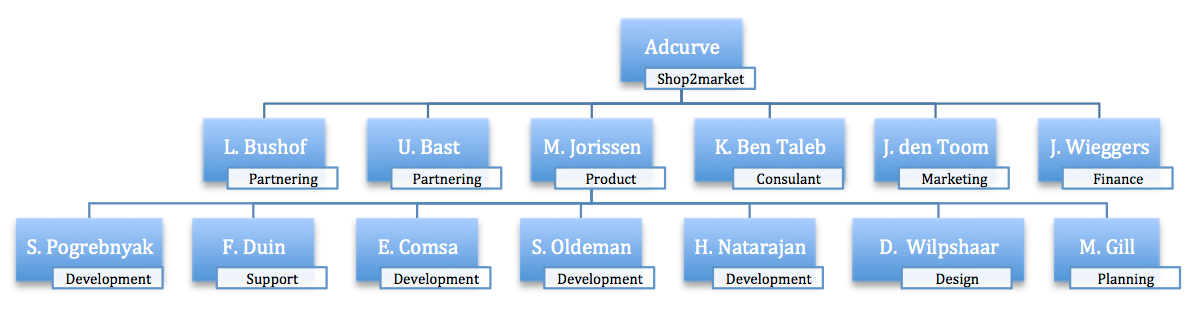
\includegraphics[width=1\textwidth]{organisation_structure.png}
    \caption{Organogram waarin het team en de relaties binnen Shop2market worden afgebeeld.}
    \label{fig:orgchart}
\end{figure}

\pagebreak

\section{De kwestie} % een kwestie (aanleiding, het op te lossen probleem, de te vervullen behoefte of de te benutten kans);

Zoals te lezen valt in de de aanleiding zijn meerdere redenen voor dit project.

\begin{enumerate}
    \item De tijd die het kost om statistieken te berekenen is aan de hoge kant. De berekeningen worden uitgevoerd met behulp van MongoDb MapReduce. Het team voorziet dat deze technologie niet genoeg schaalbaarheid bied. Dit omdat rekentijd linear is toegenomen in relatie tot de hoeveelheid data. Met de verwachte groei van Adcurve komen nieuwe requirements aan het licht en er moet naar een nieuwe oplossing worden gezocht.
    \item Bij voorkeur worden publishers geintegreerd met behulp van API's oftewijl; een externe databron. Op deze manier worden berekeningen uitgevoerd met preciese advertentiekosten. Maar doordat externe factoren nu een rol spelen in de berekeningen is het niet te garanderen dat de de uitkomst altijd correct is. Zodra fouten intern of extern hersteld zijn worden berekeningen voor een bepaalde dag, webwinkel of publisher opnieuw uitgevoerd. Het uitvoeren van dit soort correcties zijn tijdrovend door de huidge implementatie en gebruikte technieken.
    \item Als laatste onstaat er een kans door de huidige problematiek op te lossen. Webwinkels ontvangen tot soms tot 30 dagen na een bestelling een retournering van een of meerdere producten. Dit betekend dat een product niet verkocht is en de omzet uit de bestelling lager ligt dan is berekend. Het is wenselijk om berekende statestieken met betrekken tot retour bestellingen opnieuw te berekenen.
\end{enumerate}


\section{Doelstellingen} % de doelstellingen (wat moet na afloop van het afstudeerproject zijn bereikt);

In het kort moeten webwinkeleigenaren in staat zijn om beslissingen te maken op basis van correcte en actuele gegevens in Adcurve. Dit betekend dat de gegevens die Adcurve toont altijd te verklaren zijn en overeenkomen met de werkelijkheid. Als voorbeeld hiervan zijn gegevens over de vorige dag voor kantooruren beschikbaar en worden retouropdrachten ook verwerkt in Adcurve. Als laatste moeten gegevens accuraat en betrouwbaar zijn, tenzij anders vermeld staat. Daarom moet tijdig herstel van fouten mogelijk zijn.

\section{Type opdracht}

Aan de hand van beschikbare technieken wordt er gekozen een aantal mogelijk oplossingen\newline te proberen middels een Proof of Concept. Dit sluit goed aan bij de aard van een onderzoeksopdracht. Door dit onderzoek moet duidelijk gaan worden: hoe de opdracht kan worden opgelost, of dit mogelijk is en wat er nodig is om de oplossing naar productie te brengen. Door de opdrachtgever is gevraagd om een aantal POC's te ontwikkelen om tot een inzicht over de oplossing te komen. Er is hierdoor sprake van een ontwikkel opdracht.



\chapter{Onderzoeksplan}
% de onderzoeksvragen, hoofdvraag met daaruit voortvloeiende deelvragen die moeten worden beantwoord

In de kwestie zijn de problemen - beter uitdagingen te noemen - omschreven. Omdat een oplossing niet voor de hand ligt, wordt er een onderzoek opgesteld. De leidende hoofdvraag wordt in dit hoofdstuk helder.

\section{Onderzoeksvragen}
Gedurende de uitvoering van de opdracht wordt de volgende hoofdvraag beantwoord: \\
{\large \textit{"Hoe verzorgt een nieuwe implementatie voor het up-to-date houden van statistieken in Adcurve zodat gegevens altijd te verklaren zijn?"}} \\

Om de hoofdvraag te beantwoorden zijn de volgende deelvragen geformuleerd:
\begin{enumerate}
\item Wat zijn de functionele en niet functionele eisen waaraan de oplossing moet voldoen?
\item Wat zijn toonaangevende methodes en technologieën om statistieken te berekenen, die zowel passen bij de wensen en eisen van de opdracht?
\begin{enumerate}
    \item Hoe kan de opdracht worden opgelost?
\end{enumerate}
\item Welke scenario's komen met regelmaat voor waardoor gegevens niet te verklaren zijn?
\begin{enumerate}
    \item Wat zijn de gerelateerde technische factoren waardoor de scenario's voor verhindering zorgen in de huidige situatie?
    \item Wat zijn de mogelijke strategieën en technieken om dit op te lossen?
\end{enumerate}

\item Wat zijn de gepresenteerde oplossingen en waarom zijn deze volledig of niet?
\end{enumerate}

\section{Literatuur} %  (optioneel) een beschrijving van de belangrijkste literatuur die onderzocht zal worden

Voorbeelden van mogelijk jargon die zullen voorkomen in de thesis zijn data aggregaties, data transformaties en het selecteren en installeren van big data tools. Deze concepten worden onderlegd door onder andere de volgende literatuur:

\begin{itemize}
    \item Data Mining, Concepts and Techniques \parencite{data-mining}
    \item I <3 Logs, Event data, stream processing, and data integration \parencite{logs}
    \item Fast Data Processing with Spark \parencite{spark}
    \item Real-Time Big Data Analytics \parencite{realtime-architectures}
\end{itemize}

Tijdens de selectie wordt mogelijk gebruik gemaakt van verschillende fases uit “de Berenschot-methode” \parencite{cuppen}.
Daarnaast zal tijdens het voeren van gesprekken, interviews en presentaties binnen de organisatie mogelijk gebruik worden gemaakt van de theorie uit “Adviseren als tweede beroep, resultaat bereiken als adviseur” \parencite{adviseren}.

\newpage

\section{Onderzoek methode} % de te gebruiken methoden/technieken/middelen (ook van het onderzoek) en, indien van toepassing, de

% \section{Deelvragen} deelvragen voorkomend uit de gekozen ontwerpmethode (optioneel);

Voor qualitatief onderzoek wordt een \textit{Case studie} gebruikt om de problemen in de gegeven context te analyseren. Methodes binnen dit type onderzoek zijn: explanatory, descriptive en exploratory. \parencite{john-dudovskiy}. Het onderzoek is ontworpen om de fases van een Case study uit te voeren. Het ontwerp is omschreven in tabel \ref{tab:onderzoekmethode}.

\begin{center}
\begin{table}[bh]
% \centering
\caption{Onderzoek methodes met te gebruiken methoden/technieken/middelen per deelvraag}
\label{tab:onderzoekmethode}
\def\arraystretch{1.5}
\begin{tabular}{|l|p{4cm}|p{2cm}|p{2.5cm}|p{4.5cm}|}
\hline
% \rowcolor{lightgray} 
\textbf{\#} & \textbf{Deelvraag} & \textbf{Type vraag} & \textbf{Methode} & \textbf{Actie / Resultaat} \\
\hline
1 & Wat zijn de functionele en niet functionele eisen, waaraan de oplossing moet voldoen?
  & Descriptive
  & Interviews
  & MosCow prioriteiten lijst en checklist samenstellen \\
\hline
2 & Wat zijn toonaangevende methodes en technologieën om statistieken te berekenen, en passen bij de wensen en eisen van de opdracht?
  & Descriptive
  & Literature-\newline research
  & Analyseren van bronnen m.b.v. van checklist wordt een shortlist samengesteld  \\
\hline
3 & Welke scenario's komen met regelmaat voor waardoor gegevens niet te verklaren zijn?
  & Descriptive
  & Interviews,\newline Literature-\newline research
  & Inventariseren op te lossen scenario 's met prioriteit d.m.v. Impact analysis \\
\hline
3a & Wat zijn de gerelateerde technische factoren waardoor de scenario's voor verhindering zorgen in de huidige situatie?
   & Descriptive
   & Literature-\newline research
   & Vergelijkingstabel huidige en wenselijke situatie met daarbij de technissche afhankelijkheden om een scenario te kunnen voorkomen \\
\hline
3b & Wat zijn de mogelijke strategieën en technieken om dit op te lossen?
   & Designing
   & Interviews,\newline Literature-\newline research
   & Door het toepassen van de vergelijkingstabel met gevonden technologieën worden mogelijke oplossingen ontworpen \\
\hline
4 & Wat zijn de mogelijke oplossingen en hoe wordt dit gevalideerd?
   & Comparative
   & Literature-\newline research,\newline group-discussion
   & Door het Analyseren van mogelijke ontwerpen en groep discussie worden er een beperkt aantal Proof of Concepts geformuleerd met eisen. \\
\hline
5 & Wat zijn de gepresenteerde oplossingen en waarom zijn deze volledig of niet?
  & Explanatory
  & Case study
  & Conclusies op basis van van verzamelde gegevens tijdens POC fase, zoals bijv. performance tests. Tabel van oplossingen met theorieën die het resultaat verklaren. \\
\hline
\end{tabular}
\end{table}
\end{center}

% \chapter{Planning} % de projectactiviteiten met een beschrijving van de onderlinge samenhang, de mijlpalen en een fasering in de tijd met een schatting van de te besteden uren voor de verschillende uit te voeren activiteiten;

\section{De opdracht} % de afstudeeropdracht met mogelijke deelopdrachten, met vermelding van de projectgrenzen en randvoorwaarden en, indien het afstudeerproject onderdeel uitmaakt van een groter project, de afbakening t.o.v. het grotere project;

\section{De projectorganisatie} % de projectorganisatie;

    \subsection{Organisatie structuur}

    De software ontwikkeling valt onder leiding van M. Jorissen. In nauwe samenwerking met M. Gill zijn zij verantwoordelijk voor de project analyse en planning. Het development team bestaat uit zes ontwikkelaars waaronder één ontwerper D. Wilpshaar.
    De architectuur wordt geleid door S. Pogrebnyak. Dit team is verantwoordelijk voor het uitwerken en oplossen van projecten. Hierbij word gebruik gemaakt van een aantal methodieken en gewoontes vanuit Agile-softwareontwikkeling, waaronder: Kanban, Daily standup, Retrospectives, Extreme Programming (XP), Test Driven Development (TDD) en Continuous integration (CI).

    \subsection{Werkwijze en methodieken}

    Ondanks dat er in de werkwijze vaak een uitgebreide planning of requirements analyse ontbreekt, word de productiviteit en software kwaliteit toch bewaakt door de principes uit XP zoals TDD. Refactoring speelt hier een grootte rol in.\parencite{refactoring-ruby}
    \footnote{“Code refactoring is het proces waarbij de structuur van bestaande code word gewijzigd zonder de functionaliteit te wijzigen”…“dit komt ten goede aan de onderhoudbaarheid van code, en creëert nieuwe architectuur of object modellen om code makkelijker te kunnen uitbreiden met nieuwe functionaliteiten“}.
    Hierdoor kan het team zich veroorloven om bij het ontwerpen en ontwikkelen van projecten minder vooruit te plannen. Software word hierdoor gevormd door de requirements voor die in huidige situatie aanwezig zijn. In tegenstelling tot het ontwikkelen met abstracties zodat software flexibel genoeg is voor latere aanpassingen en requirements. Veel planning is hierdoor niet aanwezig en technische implementatie komt vooral tot stand door TDD, brainstorm sessies. Dit is mede mogelijk doordat de omgeving de mogelijkheid bied om fouten te maken.

    \subsection{Project verantwoordlijkheden}

    Het plannen en ontwikkelen van het software project omschreven in dit documet valt onder de volledige verantwoordelijkheid van de student. De doelstellingen en requirements worden in overleg met M. Jorissen vastgelegd. In verband met overdracht en kennis deling zal er afstemming plaats vinden met S. Pogrebnyak technische aspecten. Bijvoorbeeld over de aansluiting op huidige visie en de productie omgeving en mogelijke aanpassingen of toevoegingen aan de infrastructuur.
    De student ziet het als zijn verantwoordelijkheid is om op innovatieve wijze software te ontwikkelen.


\section{Activiteiten} % de projectactiviteiten met een beschrijving van de onderlinge samenhang, de mijlpalen en een fasering in de
tijd met een schatting van de te besteden uren voor de verschillende uit te voeren activiteiten;

\section{Risico's} % de eventuele risico’s met maatregelen;

\section{Oplevering}
% twee data voor het inleveren van concepten van de scriptie (circa 6 resp. 3 weken voor de inleverdatum van

de definitieve versie van de scriptie);


\chapter{Resultaten}

In dit hoofdstuk worden alle resultaten uit het onderzoek gepresenteerd
Deelvraag 1 "Wat zijn de functionele en niet functionele eisen, waaraan de oplossing moet voldoen?" wordt beantwoord in \ref{sec:deelvraag1}

Deelvraag 2 "Wat zijn toonaangevende methodes en technologieën om statistieken te berekenen, en passen bij de wensen en eisen van de opdracht?"\  wordt beantwoord in \ref{sec:deelvraag2}

In \ref{sec:deelvraag3} wordt gekeken naar "Wat zijn de probleem scenario's waardoor gegevens niet te verklaren zijn, en wat zijn de mogelijke oplossingen?"\ 

In Deelvraag 4 is beantwoord in \ref{sec:deelvraag4} wordt belicht hoe de expirementen zijn ontworpen

Conclusies en een vergelijking wordt gemaakt in het betantwoorden van Deelvraag 5 "Wat zijn de gepresenteerde oplossingen en waarom zijn deze volledig of niet?" te lezen in \ref{sec:deelvraag5}

% MAIN QUESTION: "Hoe verzorgt een nieuwe implementatie voor het up-to-date houden van statistieken in Adcurve zodat gegevens altijd te verklaren zijn?"

\clearpage

% ACTIVITY Afleggen interviews rondom Requirements \& Constraints, documenteren use-cases
% RESULT MosCow prioriteiten lijst en checklist
\section{Functionele en niet functionele eisen}
\label{sec:deelvraag1}

Wat zijn de functionele en niet functionele eisen, waaraan de oplossing moet voldoen?

In een interview zijn de functionele en niet functionele eisen gegeven door Matthijs Jorissoen. De studen heeft 

[TODO: geef extra uitleg over de gebruikte methode MoSCoW \cite{ma2009effectiveness}]

\begin{comment}
Een functionele eis kan gezien worden als iets dat de gebruiker nodig heeft om het doel te bereiken of een bepaalde voorwaarde waaraan de oplossing moet voldoen.

Een non functionele eis is een beperking doe wordt opgelegd op een mogelijke oplossing, met het doel om functionele eisen te behalen of het doel van het project.
\end{comment}

\begin{table}[bh]
\centering
\caption{lijst van eisen geprioritiseerd met behulp van de MoSCoW analyse}
\label{table:requirements}
\def\arraystretch{1.5}
\begin{tabular}{|l|p{13cm}|}
\hline
\textbf{Prioriteit} & \textbf{Functionaliteit/Requirement}
\\ \hline
Must have           & Statistieken voor één webwinkel kunnen opnieuw worden gegenereerd zodat veranderingen in externe data bronnen bijvoorbeeld orders of geïmporteerde kosten opnieuw worden geaggregeerd. Dit moet tot 30 dagen terug.
\\ \hline
Must have           & Het creëren van data aggregatie voor alle webwinkels over een dag, mag niet meer tijd in beslag nemen dan de huidige oplossing nodig heeft. Dit is 1 uur en 30 minuten.
\\ \hline
Must have           & De kosten voor eventuele licenties en infrastructuur mogen niet hoger zijn dan dat voor de huidige oplossing vereist is
\\ \hline
Should have         & Statistieken zijn altijd voor kantoor uren beschikbaar voor het dashboard en latere processen zoals tips generatie
\\ \hline
Should have         & De gekozen oplossing heeft een productief programmeermodel en uitvoerbaar op niet afhankelijk van een hardware architectuur
\\ \hline
Could have         & De programmatuur is testbaar en hierdoor eenvoudig te onderhouden
\\ \hline
Could have          & Data aggregaties voor een groep webwinkels kunnen op een ander tijdstip worden geaggregeerd i.v.m. verschillende tijdszones
\\ \hline
Could have         & De nieuwe oplossing moet schaalbaar genoeg zijn om 10.000 klanten te kunnen onderstuenen.
\\ \hline
\end{tabular}
\end{table}

Een aantal gebruikte termen zoals simpel, snel etc. worden verduidelijkt met de bijbehorende definities die in overleg tot stand zijn gekomen: \\

\begin{itemize}
    \item \textbf{Een productief programmeermodel} in de context van een dit project wordt omschreven in \cite{asanovic2006landscape}: "programming models should be independent of the number of processors, they should allow programmers to use a richer set of data types and sizes, and they should support successful and well-known parallel models of parallelism"

    \item \textbf{Scalability} wordt door \cite{dubey2005recognition} gefefineerd als: Schaalbaarheid is het vermogen om de gewenste snelheid te bieden en te onderhouden al dan niet verbeteren. De industrie hier twee manieren voor. "Scale up" is de methode waarbij hardware wordt vervangen zodat er betere prestatie geleverd kan worden. Bij "scale out" wordt er extra hardware aangesloten zodat een bestaand systeem de toenemende werkdruk kan ondersteunen.
\end{itemize}

\begin{comment}
De grootte van alle databronnen voor een webwinkel per dag ligt tussen de 0.5 MB en 130 MB per dag. Om de data grootte in te schatten met 10.000 webwinkels kan huidige datagrootte van een gemiddelde dag worden ge-extrapoleert. Er moet rekeningen worden gehouden met het Paretoprincipe, dat zou verklaren dat 20\% van de webwinkels verantwoordelijk is voor 80\% van de datagrootte. Dit is ook waar te namen in het analyseren van de datasets. % https://en.wikipedia.org/wiki/Pareto_principle

\end{comment}

\clearpage

% ACTIVITY Onderzoeken van toonaangevende, passende technologieën
\section{Toonaangevende methodes en technologieën}
\label{sec:deelvraag2}

Wat zijn toonaangevende methodes en technologieën om statistieken te berekenen, en passen bij de wensen en eisen van de opdracht?

Uit verschillende bronnen zijn richtingen gevonden voor mogelijke oplossingen. Zoals het gebruik van database oplossingen, distributed oplossingen, en hardware oplossingen.
\footnote{
Uit de volgende opgevraagde webpagina's zijn verschillende onderzoeksrichtingen gevonden. De github pagina heeft over 200 technologieën en referenties naar verschillende papers.
\begin{enumerate}
    \item \url{https://github.com/onurakpolat/awesome-bigdata}
    \item \url{https://experfy.com/blog/hadoop-market-size-adoption-growth-2020/}
    \item \url{https://cs.arizona.edu/~bkmoon/papers/sigmodrec11.pdf}
    \item \url{http://datanami.com/2014/11/21/spark-just-passed-hadoop-popularity-web-heres/}
    \item \url{http://radar.oreilly.com/2014/01/a-compelling-family-of-dsls-for-data-science.html}
\end{enumerate}
}


\subsection{Databasese oplossingen}

De volgende lijst van database systemen beschikken over analytical functionaliteiten nodig voor het aggregeren en creeëren van statestieken. Voor het maken van data aggregaties zijn baisis SQL functies nodig: SUM, MIN, MAX, AVERAGE, samen met de SQL clauses: GROUP BY en HAVING. Omdat bijna alle database systemen deze functies onderstuenen is er gekeken naar databases die een hoog volume aan data kunnen verwerken. 
Omdat er nu per dag zo'n 1.8Gb aan data voor alleen visits wordt verwerkt en dit extropaleert naar (1.8/480) * 100000 = 375Gb per dag. \\

Traditionele databases systemen zijn gemaakt om transactionele queries te beantwoorden. Deze zullen minder schaalbaar zijn doordat er verschillende fases zijn die overhead introduceren. \parencite{harizopoulos2008oltp}
Daarnaast introduceert het frequent updaten en corrigeren data bronnen mogelijke performance problemen doordat data consistentie wordt gegarandeerd met methodes als "table locks". Verder raken databases overbelast wanneer de opgravraagde database query resulteert in een dataset die nit in het geheugen is te plaatsen.  daarom tot een trager, overbelast systeem. \parencite{kersten2011researcher} \\

Database queries kunnen overigens erg traag raken wanneer databases groeien en query resultaten niet meer in RAM passen. Hierbij wordt resulteert een terugval op de hardeschijf (zogeheten "Disk spills") in het vertragen van een datapipeline. Ook zijn er verschillende anakedotes vanuit de organisatie waarbij databases zoals MySQL sporadisch, overbelast raakt.

%"Moreover, database queries often contain blocking operations that lead to a pipeline stall or spilling large intermediates back to the disks." \parencite{kersten2011researcher}


Het plan in onze use-case is om frequent data aggregaties uit te voeren zodat statestieken in adcurve worden gecorrigeerd. Dit kan er uiteindelijk voor zorgen dat locking systemen om data consistentie te garanderen een bottle neck op a 
Traditionele databases garanderen waarbij een transactionele niet worden beschouwd als een verkiesbare technologie. Daarom is gekeken naar databases met een andere storage engine.  \\

Opvallend is dat bijna alle distributed en analytics databases van PostgreSQL afstammen \parencite{postgresforks}

Hieruit valt te concluderen dat de business intelligence industry veel research heeft geinvesteerd in op basis van Postgress technology. \\

Michael Stonebraker is origineel auteur Postgress en later vele high performance databases. In zijn paper "How To Build a High-Performance Data Warehouse"\  omschrijft hij drie verschillende architectuur typen / storage engines: Shared Memory, Shared Disk en Shared Nothing.
"Because shared nothing does not typically have nearly as severe bus or resource contention as shared-memory or shared-disk machines, shared nothing can be made to scale to hundreds or even thousands
of machines. Because of this, it is generally regarded as the best-scaling architecture". \parencite{dewitt2006build}



In de paper worden de volgende databases genoemd:
\begin{table}[bh]
\centering
\caption{My caption}
\label{my-label}
\begin{tabular}{|l|l|l|}
\hline
\textbf{Shared memory} & \textbf{Shared Disk} & \textbf{Shared Nothing} \\ \hline
Microsoft SQL Server   & Oracle RAC           & Teradata \\
\hline
PostgresSQL            & Sysbase IQ           & Netezza \\
\hline
MySQL                  &                      & IBM DB2 \\
\hline
                       &                      & GreenplumDB \\
\hline
                       &                      & Vertica \\
\hline
\end{tabular}
\end{table}
\clearpage

\subsection{Distributed oplossingen}
In 2009 werd geconstateerd door \cite{aarnio2009parallel} werd MapReduce als geidentificeerd als een "Prominent parallel data processing tool" dat tractie kreeg vanuit zowel de industrie als de academische wereld. Zo concludeerde zij dat: "Naast traditionele Database Management Systems is Map Reduce een zeer schaalbaar en flexibele oplossing is voor een variatie aan data analyses" \parencite{aarnio2009parallel}

Voor langere tijd nu, staat Hadoop bekende als een volwasse technologie en implementatie van Map Reduce, zo schrijft Gartner in een recent rapport: "The open-source software framework known as Apache Hadoop has gained sizable acceptance in organizations, spurred on by the growing digital business appetite for big data" \parencite{hadoop2013selection}.


"Joe Hellerstein, our local expert in databases, said the future of databases was large data
collections typically found on the Internet. A key primitive to explore such collections is
MapReduce, developed and widely used at Google \parencite{dean2008mapreduce}" \parencite{asanovic2006landscape}, 

Kort nadat UC Berkley zijn cluster framework "Spark" heeft gedoneerd aan de Apache foundation in 2014, heeft het project enorme aandacht ontvangen vanuit de hele industrie. \parencite{spark2015intro}. Zo is er ook vanuit Shop2market enorme interesse in Apache Spark. Er zijn al eerder in 2015 Proof of Concept uitgevoerd met betrekking tot machine learning applicaties.

Terwijl nog veel organisaties zweven tussen het begrijpen en het vinden van de toepassing voor Hadoop \parencite{hadoop2015adoption}, is sinds 2013 een alternatief in memory implementatie van o.a. Map reduce enorm populair  \parencite{spark2015intro}

\subsubsection{\textbf{Conclusie}}

De uiteindelijke selectie voor dit onderzoek is beperkt. De frameworks die zijn geselecteerd hebben genoeg herkenning vanuit de organisatie en industrie. De enorme lijst op github is getuige van de enorme hype rondom Big Data. Toch zijn veel organisaties nog zoekend naar wat technologie betekent en hoe het waarde toevoegd\parencite{hadoop2015adoption}.

Verder zijn er in de eerder genoemde lijst (github) enorm veel tools benoemd. In dit onderzoek zullen naast Hadoop en Naast eerder besproken frameworks Spark en Hadoop zijn er andere technologieën waar colleg's eerdere ervaring mee hebben.

De selectie van technologieën komt uit op

\begin{itemize}
    \item Disco
    \item Apache Flink
    \item Hadoop (Apache MapReduce)
    \item Apache Spark
\end{itemize}

Streaming methodes zoals bijvoorbeerld Apache Storm worden als toonaangeevend gezien maar zijn niet geselecteerd. Dit omdat de vorm waarin de data beschikbaar wordt gesteld aan het aggregatie proces altijd in batch is. Het valt buiten de scope om deze data flows te veranderen.
\clearpage

\subsection{Hardware oplossingen}
Een van de oplossingen die wordt onderzocht is het gebruik maken van krachtige hardware componenten (zowel de CPU en de GPU). Dit is mogelijk met expert talen zoals; Verilog, CUDA of OpenCL of C++.


Op de universiteit van Stanford is hier veel onderzoek naar gedaan. Dit vereist alleen veel hardware specifieke kennis en moet in code worden uitgedrukt: "programming these devices to run efficiently and correctly is difficult, error-prone, and results in software that is harder to read and maintain." \parencite{sujeeth2011optiml}. Daarom is er een serie aan DSL's ontwikkeld\footnote{Voorbeelden van DLS 's zijn \TeX, HTML en SQL  \parencite{sigplan2000dsl}}

Terwijl \textcite{sujeeth2011optiml} een veelbelovende oplossing lijkt aan te bieden is het project nog altijd in Alpha versie \parencite{optiml_project_home}. Hetzelfde team presenteerde in 2014 Forge, een DSL voor expert talen met veelbelovende test resultaten: "Forge-generated Delite DSLs perform within 2x of hand-optimized C++ and up to 40x better than Spark" \parencite{sujeeth2014forge}. Helaas lijkt hierbij hetzelfde probleem te spelen en is er niet genoeg documentatie gevonden om hier een POC mee te starten.

Binnen Shop2market zijn veel performance gerelateerde projecten opgelost met Golang. Naast dat dit erg productief is bevonden biedt de moderne taal een alternatief concurrency model. "C, C++, and to some extent Java are quite old, designed before the advent of multicore machines, networking, and web application development. There are features of the modern world that are better met by newer approaches, such as built-in concurrency." \parencite{pike2012go}.

\subsubsection{\textbf{Conclusie}}

De besproken technologieën zijn de DSL talen: OptiML, OptiSQL en Forge. Bij gebrek aan praktische voorbeelden en algemene documentatie is er voor gekozen om hier niet verder in te investeren. Er zou niet voldoende kennis zijn om een mogelijke POC naar productie te brengen. Hoewel Forge tijdens de benchmarks extreem goed presteert, wordt niet vermeld welke algoritmes hierbij zijn gebruikt. Omdat in de huidige implementatie gebruik wordt maakt van MapReduce (de Monte Carlo methode) hoeft deze performance niet behaalt te worden. Zo schrijft \textcite{lee2010debunking}: "Monte Carlo algorithms are generally compute-bound with regular access patterns, which makes it a very good fit for SIMD architectures", in vergelijking met een GPU processor. Golang biedt hier een mogelijke oplossing, omdat de taal een productieve manier biedt om optimaal gebruik te maken van Multicore CPU's.

\clearpage

% ACTIVITY Impact analyse uitvoeren rondom use-cases
\section{Problematische scenario 's en mogelijke oplossingen}
\label{sec:deelvraag3}
\textit{Wat zijn de probleem scenario's waardoor gegevens niet te verklaren zijn, en wat zijn de mogelijke oplossingen?}

Tijdens de project analyse is met verschillende stakeholders binnen de organisatie gesproken. Naast de gedefinieerde projecteisen zijn er verschillende symptomen verzameld. Deze zijn gebruikt voor het samenstellen van een Impact analyse gemaakt, zie Apendix \ref{app:impact_analyse}

Vervolgens is per probleemscenario een mogelijke technische verklaring gezocht, zijn er criteria omschreven waaraan de gebruikte technologie bij een mogelijk oplossing moet voldoen. Hierdoor wordt getoetst of de geselecteerde technologieën in \ref{sec:gevonden_tools} toepasbaar zijn en de huidige probleem scenario werkelijk kunnen oplossen.

\subsection{Scenario's uit de Impact Analyse}

\begin{enumerate}
    \item L6: API 's provided by the publisher are unavailable
    \item M5: API 's for google, change frequently and the import stops working, or fail silent (values are not matched,,resulting in empty fields)
    \item H6: Wrong costs by configuration, issues: mistakes in tracking Order amount, tracked wrong, multiplied by 100 bug
    \item L7: Metrics calculated incorrectly because of mismatching product data (ids from tracking don't match cost exports from publisher)
    \item L7: Calculations fail,because technology or infrastructure 
    \item L4: Aggregations from different dimensions on the same data
    don't match
    \item H7 Bij het bekijken van dashboards in Adcurve zijn de gegevens over de vorige dag pas beschikbaar na 12:30 CET. Omdat alle data in een keer wordt verwerkt wordt het proces gestart nadat alle afhankelijke data bronnen beschikbaar zijn.
\end{enumerate}

Scenario een (1) tot en met vier (4) zijn niet te voorkomen omdat de organisatie zelf hier weinig invloed op kan hebben. Het wordt veroorzaakt door externe processen bij publishers, of mensen in diesnt van de webwinkel die de advertenties of webwinkel integraties verkeerd configureren. Scenario vijf (5) en zes (6) hebben een hoge impact en zijn specifieke problemen met de huidige implementatie. Deze scenario's zijn te voorkomen door het inzetten van andere technologie of een andere strategie als het aan komt op data processing.
Scenario 7 is eerder besproken tijdens de non functionele eisen in \ref{table:requirements}. Deze is opgenomen zodat onderzocht wordt hoe dit het best kan worden voorkomen.  

\clearpage

\subsection{Technische te verklaren oorzaken}

Met betrekking tot scenario vijf (5) en zeven (6) zijn verschillende problemen gevonden in relatie tot de gebruikte versie van MongoDB \parencite{mongo_changelog}. Uit monitoring systemen zijn de foutmeldingen terug te relateren aan software bugs die aanwezige zijn in versie 2.4.

De consensus binnen de organisatie is dat een upgrade naar een volgende versie riskant is. Het is niet in te schatten hoe veel problemen er zullen optreden. Daarnaast moeten er processen worden ingericht om het synchroniseren van order te ondersteunen en data verlies te voorkomen wanneer de database offline moet.
% TODO: is het mogelijke om machines van verschillende versies naast elkaar te draaien in een cluster?
    
Met betrekking tot scenario zeven (7) zijn de volgende mogelijke oorzaken gevonden:

\begin{itemize}
    \item Uit monitoring systemen blijkt dat het online productie processen van invloed zijn op de performance van het aggregatie proces. Omdat MongoDB direct wordt gebruikt voor het synchroniseren van bestellingen met webwinkels, en dit een realtime proces is, wordt het cluster hiermee belast. In de huidige situatie worden de MapReduce jobs op een aantal machines in het cluster uitgevoerd, toch word de performance beïnvloed.
    \item het aggregeren van data kan in MongoDB wellicht trager zijn dan nodig omdat de tussentijdse resultaten uit de fases in MapReduce worden weggeschreven naar verschillende machines \parencite{mongo_mr_shards}. Zo valt ook af te lezen uit monitoring dat het wegschrijven van de uiteindelijk resultaten langer duurt dan het aggregeren zelf. Dit heeft mogelijk te maken met het bijhouden van indexes.  \parencite{mongo_write_performance}
    % replica sets? sharding? grootte cluster?
\end{itemize}


\subsubsection{\textbf{Conclusie}}
\label{subsec:3.3.2}

Tijdens de root cause analysis zijn een aantal oorzaken omschreven. Hieruit valt te concluderen dat een mogelijke nieuwe oplossing aan de volgende criteria moet voldoen:

\begin{enumerate}[label=(\alph*)]

    % Er rekening moet worden gehouden met de mogelijke overhead van networking applications, en tegelijkertijd de mogelijkheid moet zijn om grootte data sets op te splitsen zodat er geen ``disk spills"\ optreden.
    \item In de nieuwe situatie moet op efficiënte wijze worden om gegaan met een kleine hoeveelheid aan data, zodat de verschillende fases van het aggregeren (zoals map, reduce, shuffle en sort). Dit omdat voor 80\% van de webshops een kleine hoeveelheid data wordt verzameld. Tegelijkertijd is de input data set groot en zijn resultaten van aggregaties wellicht groter. Er moet in deze situatie op efficiënte wijze data worden weg geschreven naar een eindlocatie,  zoals het filesysteem. Hierbij moet het onderhouden van indexes worden voorkomen.
    
    \item Er moet situaties situatie worden voorkomen waarin het onmogelijk is om een technologie of systeem te upgraden naar een nieuwere versie. Dit is te voorkomen door a) geen state te bewaren in het systeem zelf, maar dit alleen te gebruiken bij data processing. b) door het systeem onafhankelijk te maken van productie / online processen. Dit biedt de mogelijkheid door bijvoorbeeld een database back-up te doen, het systeem te migreren en de data opnieuw in te laden.
\end{enumerate}

\clearpage


\subsection{Hoe wordt dit voorkomen met de gevonden tools / POC?}
\label{subsec:deelvraag3_vergelijking}


\subsubsection{\textbf{Versie upgrades}}

Door de tools binnen het Hadoop ecosysteem wordt geen state bewaard. Maar alle data wordt beheerd door HDFS en opgeslagen als toegankelijke bestanden in een gekozen bestandsformaat. Het risico is dat het upgraden van versies, niet compatible met verschillende bestands formaten. Ook de tools die opereren op het data formaat moeten compatible zij. Daarnaast bestaat de mogelijkheid dat HDFS data anders beheerd onder verschillende versies. Hierdoor zijn data migraties erg operationeel intensief is. Hierdoor is het sterk aan te raden om dit niet zelf te beheren, maar gebruik te maken van distributie zoals Amazon EMR, Hortonworks, Cloudera of MapR.

Omdat Spark onder andere uitmaakt van het Hadoop ecosysteem zijn deze conclusies te generaliseren.

Omdat databases bij definitie statefull zijn, moet er in dit geval een back-up en restore mogelijkheid aanwezig zijn om upgrades te kunnen uitvoeren.

In het geval van Golang, dat in het algemeen niet als data processing tool te beschouwen is maar als een General purpose language, is de implementatie code eenvoudig te upgraden naar nieuwere versies. Dit wordt gegarandeerd als de implementatie volledig getest is door unit tests. 


\subsubsection{\textbf{Mogelijke overhead voorkomen}}

\begin{verbatim}

Use the COST PAPER (single threading vs. network overhead)

https://www.usenix.org/conference/hotos15/workshop-program/presentation/mcsherry

AND The paper measuring NETWORK OPTIMIZATIONS vs CPU/MEM in DATA PROCESSING TOOLS VS CPU
https://www.usenix.org/system/files/conference/nsdi15/nsdi15-paper-ousterhout.pdf

Reference to the paper and explain:
SPARK USES NO INDEX \parencite{armbrust2015spark}
MAP REDUCE (Google / Apache) USES NO INDEX 
SHARED NOTHING DATABASES USE NO INDEXES \parencite{lamb2012vertica} of \parencite{harizopoulos2008oltp} / \parencite{dewitt2006build}

MAYBE ALSO APPLY 'Amdahls law'
https://en.wikipedia.org/wiki/Amdahl%27s_law

 AND MAYBE 
"roughly 80\% of the effects come from 20\%"
https://en.wikipedia.org/wiki/Pareto_principle

\end{verbatim}


\subsubsection{\textbf{Oplosing om  high query speed en good analytics performance te behalen met  twee losse systemen}}

Het splitsen van data verwerken en data opslag / opvragen betekend dat de geaggregeerde data zal worden opgeslagen in s3, zodat de bestaande API de data kan uitserveren. 
De aggregaties op basis van week, jaar en maand komen te vervallen. De overige aggregatie die nodig is om API client snel te houden wordt gedaan door Saki. Doordat de bestanden gesorteerd worden opgeslagen op s3, kan saki deze binnen 100 milliseconden aggregeren per query.

Dit heeft als gevolg dat data opslag volledig verplaatst naar Amazon S3, zowel de input data als de output data. (data pipeline)

    
\subsection{Conclusie}

Een deel van het probleem is het actief monitoren van de data kwaliteit en processen starten om het te corrigeren. Hier wordt niet verder op in gegaan omdat een dergelijke oplossing hiervoor buiten scope valt. Hiervoor geldt, zodra er een oplossing is moeten de datakwaliteit worden herstelt door het proces te starten dat de correcties uitvoert [``effected datasources"\ opnieuw evalueren]
Deze scenario's zijn ook tegelijkertijd lastig te voorkomen, alleen te herstellen. Het advies is daarom om hier ``monitoring en alerting\ voor te implementeren en verder onderzoek doen naar bestaande methodieken voor beheersen van datakwaliteit. Bijvoorbeeld door starten van een ``Data Stewardship Program" zoals omschreven wordt in het ``TDWI Report, The Data Warehouse Institute"\ door  \textcite{eckerson2002data}.

Spark SQL is bewezen snel erg snel te zijn en Amazon EMR is managed service

database column store heeft geen indexes maar partities, bewezen erg snel te zijn… maar geen voordelen worden behaald omdat  ons proces altijd N-max aantal columns worden opgevraagd. Daarom zal de query nooit sneller zijn, unless er meerdere query 's zijn waarbij verschillende columnen worden opgevraagd. Daarom zijn er te weinig voordelen om hier een POC mee te starten, daarnaast zullen versie upgrades lastig zijn. 

De Aggregatie processen met Golang zullen erg klein worden gemaakt door de data van te voren te partitioneren per shop. Dit biedt de mogelijkheid om het deze processen uit te voeren op verschillende machines (scale-out), door het gebruikt van resqueue workers "Resque workers can be distributed between multiple machines, support priorities, are resilient to memory bloat / "leaks," \parencite{github2016reque} 


Kort: Er wordt niet verder geïnvesteerd in een POC met databases omdat er te veel keuze is, en technologie niet effectief is toe te passen

Wel wordt er een POC uitgevoerd met Golang en Spark


% Het splitsen van data verwerken en een databases waaruit de data is op te vragen, heeft met gevolg dat Saki, een applicatie die in real time aggregaties op het hoogste niveau pakt (channel, shop, shop_product_id) en deze flexibel aggregeerd op basis van datum.
\clearpage


% ACTIVITY Bespreken van ontwerpen en evt. aanpassen van ontwerpen
% ACTIVITY Vastleggen kwaliteitscriteria Proof of concept's
\section{Ontworpen experimenten middels proof of concept}
\label{sec:deelvraag4}
% \textbf{Hardware oplossing met Golang}
% Het is praktisch mogelijk om data in sub sets te aggregeren omdat er een afzonderlijke data bron is per publisher.
% Het gebruiken van gesplitste bestanden per webshop zorgt voor zeer korte levende processen. De totale performance hoeft niet te verbeteren, zolang het proces dat alleen data aggregatie uitvoert voor de specifieke webwinkel en publisher kort van duur is kan dit worden uitgevoerd op verschillende machines tegelijk om dit schaalbaar in te zetten. "We typically find that the highest performance is achieved when multiple threads are used per core. For Core i7, the best performance comes from running 8 threads on 4 cores" \parencite{lee2010debunking}

% \textbf{Distributed oplossing met Spark}
% Door gebruik te maken van distributed functionaliteiten van Spark wordt getest of de snelheid waar spark bekend om staat (paper) behaald kan worden in onze use case. Er is de mogelijkheid om unit tests en functional tests te schrijven, dit wordt aangeboden door het framework. Het wegschrijven van meerdere resultaten in een proces kan door het partitionener van output data op (PublisherID, ShopID). Ook kunnen er meerdere dagen in een proces worden verwerkt en het resultaat wordt weggeschreven per TimeID, PublisherID en ShopID


In dit hoofdstuk worden gepresenteerd hoe de POC / expirimenten zijn ontworpen. Zoals is te lezen in \ref{sec:deelvraag3} is zijn de best mogelijke oplossingen te ontwikkelen met behulp van \textit{Golang} en \textit{Apache Spark}. In overeenstemming met de organisatie zijn verdere succesfactoren gedefinieerd per POC.


% De uitvoer van het project bestaat uit drie fases; Data preperation, Go Aggregate en Spark SQL
% In fase 1 vindt de ETl processing plaats. Als de resultaten snel genoeg zijn, zal dit worden hergebruikt in fase 2 en 3.
% TODO Leg uit dat Spark SQL niet wordt aangeraden voor ETL wanneer dit alleen mapping fases heeft


\subsection{Ontworpen expirimenten}

Zoals wordt omschreven in de originele doelstelling in \ref{sec:doelstelling} ``moet data op tijd worden verwerkt evenals het tijdig herstellen van fouten mogelijk zijn".  Daarom valideert dit expiriment welk POC beter presteert gegeven de huidige context. Voor het meten van de prestaties worden er drie vershillende type aggregaties uitgevoerd op "Commodity hardware", de exacte specificaties worden later omschreven in sectie \ref{subsec:3.4hardware_specs}.  Er wordt gebruik gemaakt van een productie data set van één willekeurige dag.

Tijdens iedere aggregatie worden er twee metingen: de totale proces \footnote{tijd word gemeten door unix \verb#time# zie de documentatie voor time: \url{http://linux.die.net/man/1/time}} en de totale tijd zonder de warmup time.  Warmup time wordt in dit expiremnt omschreven als de tijd die nodig tussen het starten van het proces en het werkelijk uitvoeren van de geschreven implementatie. Dit zal worden toegelicht per POC.

Voor het evalueren van de twee POCs is besloten om geen latency, IO, memory of CPU gerelateerde benchmarks te evalueren. Veelal omdat dit inzicht in geeft in prestaties van de hardware. En omdat door de  academia en industry veel energie investeerd in het verbeteren van performance van bijv. data processing tools zoals hadoop en spark. Voor de doelstellingen van het project (in dit stadium) is de totale proces tijd belangrijker.

\subsection{Gebruikte data sets}

Tijdens de drie fases van het expirement wordt inconsistent gebruik gemaakt van een data set uit productie als data input. De data set bestaat uit visits en orders van 264 webwinkels uit de benelux.

\begin{itemize}
    \item Het \textbf{Orders} bestand is origineel 0.2494 GB groot, dit is in een Binary JSON (BSON) compressie formaat, Na het ETL waarbij alleen de alleen de relevantie metrieken overblijven is de dataset 0.04734 GB groot. Dit is een JSON formaat waarbij alle extra colommen voor visits ook zijn inbegrepen en een default waarde hebben.

    \item Het \textbf{Visits} bestand is orgineel 1.0GB groot, dit is in een CSV bestand waarbij de TAB charachter als delimiter wordt gebruikt.  Na het ETL waarbij alleen de alleen de relevantie metrieken overblijven is de dataset 0.04734 GB groot. Dit is hetzelfde JSON formaat waarbij alle extra colommen voor orders zijn ingebrepen en een default waarde hebben.
\end{itemize}

Het resultaat van de ETL voor orders en visits wordt als input data gebruikt voor iedere aggregatie. De drie aggregaties zijn variaties waarbij dezelfde input data wordt gebruikt, maar waarvan het resultaat verschilt per aggregatie in data grootte. Dit is om de huidige situatie en business needs te simuleren. Een grotere data set past wellicht wel of niet in het geheugen (RAM). De drie variates maken gebruik van de volgende keys waarop de aggregatie functie \verb#SUM(metric)# wordt toegepast:

\begin{itemize}
    \item TimeId, ChannelID
    \item TimeId, ChannelID, ShopId
    \item TimeId, ChannelID, ShopId, ShopProductId
\end{itemize}

Ieder opdracht (aggregatie) wordt in één serie vijf keer herhaalt, waarvan een vervolgens de twee metingen worden geregistreerd. Over de metingen wordt een gemiddelde genomen.

\subsection{ETL Process, Data preperation}

De eerste fase uit het algoritme is een ETL stap, om csv en bson te converteren naar een uniform schema.
dit heeft de volgende voordelen
% de visits (csv) dump uit Cassandra, orders (bson) dump uit MongoDb, Geïmporteerde advertentiekosten van diverse publishers (csv)


download data sets, unzip, run splitter. bson naar json en csv naar json.
de structuur van orders bson is als volgt

de structuur van visits bson is als volgt

dit resulteert in het volgende schema
data wordt weg geschreven in bestanden per webwinkel
dit heeft de volgende reden / voordelen
% als een methode om eenmalig te filteren i.p.v. meerdere malen tijdens het aggregatie proces.


\subsection{Golang}

- wat zijn de eisen die zijn besproken

- de oplossing is als volgt ontworpen

- de gevonden resultaten

- warmup time is in gecompileerde Go code niet van toepassing.
Omdat Golang compileerd naar assembly is er geen sprake van warmup time

\subsection{Spark}

- wat zijn de eisen die zijn besproken

- de oplossing is als volgt ontworpen

- de gevonden resultaten

- warmup time
De warmup tijd in spark is te verklaren doordat de Spark SQL syntax wordt veraalt naar Java, het de java code wordt vertaal naar systeem code door de JVM.


\subsection{De setup}
\label{subsec:3.4hardware_specs}








\clearpage

% ACTIVITY Uitvoeren van Proof of concept's
\section{deelvraag 5 - Conclusies}
\label{sec:deelvraag5}
Wat zijn de gepresenteerde oplossingen en waarom zijn deze volledig of niet?

\textbf{Go Aggregator}
Split all orders and visits for all shops (264 shops)

\begin{lstlisting}
2016/05/11 11:38:45 Begin
2016/05/11 11:40:09 Main Done
./start.sh  69.83s user 16.12s system 101% CPU 1:24.70 total

total time: 1 minute 9 seconds
\end{lstlisting}

\textbf{Spark all shop products, file per shop}

(one file contains all products for all channels)

\begin{lstlisting}
16/05/11 10:09:58 INFO SparkContext: Running Spark version 1.6.0
[2016-05-11 10:10:03] Start loading data
[2016-05-11 10:12:24] Finished writing data
Total time:     0:02:21.378717
16/05/11 10:12:24 INFO ShutdownHookManager: Deleting directory /private/var/folders/tp/….

time without job submit: 2 minutes 21 seconds
\end{lstlisting}


\textbf{Conclusie}

[todo]

Het gebruik van big data systemen is zeer schaalbaar, maar introduceerd een hoop overhead. (paper).

Voordelen van een programmeer taal is dat complexe business logic hierin kan worden geschreven zonder rekening te houden met veel abstracties zoals in parallel programming zoals map reduce of sql.. In zo'n paradigm moet een probleem naar code worden vertaalt met extra kennis naast het programmeren, kennis over het map reduce paradigm, sql join. Daarnaast wordt code vertaalt naar een query plan en het gebruik van indexes etc..



%% Use letters for the chapter numbers of the appendices.
\appendix

% 
\chapter{Overzicht planning en fases}
\label{app:planning}

In de volgende twee pagina's zijn de planning en fases in meer detail omschreven\footnote{ Deze pagina's zijn in het engels geschreven, omdat dit de voertaal is binnen het bedrijf }. De onderzoekmethode, zie tabel \ref{tab:onderzoekmethode} op pagina \pageref{tab:onderzoekmethode}, dient als basis voor deze planning.
\newline

In de "Breakdown structrure, estimates per activity"\ wordt inzichtelijk gemaakt hoe de tijd is onderverdeeld per activiteit en Proof of concept. Er wordt rekening gehouden met de mogelijke risico's en daarom kan in werkelijkheid de uitvoering sneller dan hier ingepland.

In de lijst met lijst met activiteiten, zie sectie \ref{sec:activiteiten} op pagina \pageref{sec:activiteiten}, zijn de inschattingen in uren geschreven. Echter zijn de inschattingen origineel gedaan in dagen, omdat dit beter aansluit bij de werkwijze van Shop2market. Dit wordt dan ook gehanteerd in apendix \label{app:planning}.
\newline

In "Visualisation in calendar days based on estimates per activity"\ is te zien hoe de planning past binnen de iteraties bij Shop2market, aansluitend bij de werkwijze in de organisatie. Andere belangrijke momenten als inleverdata en concept versies van de thesis zijn hier ook in opgenomen.

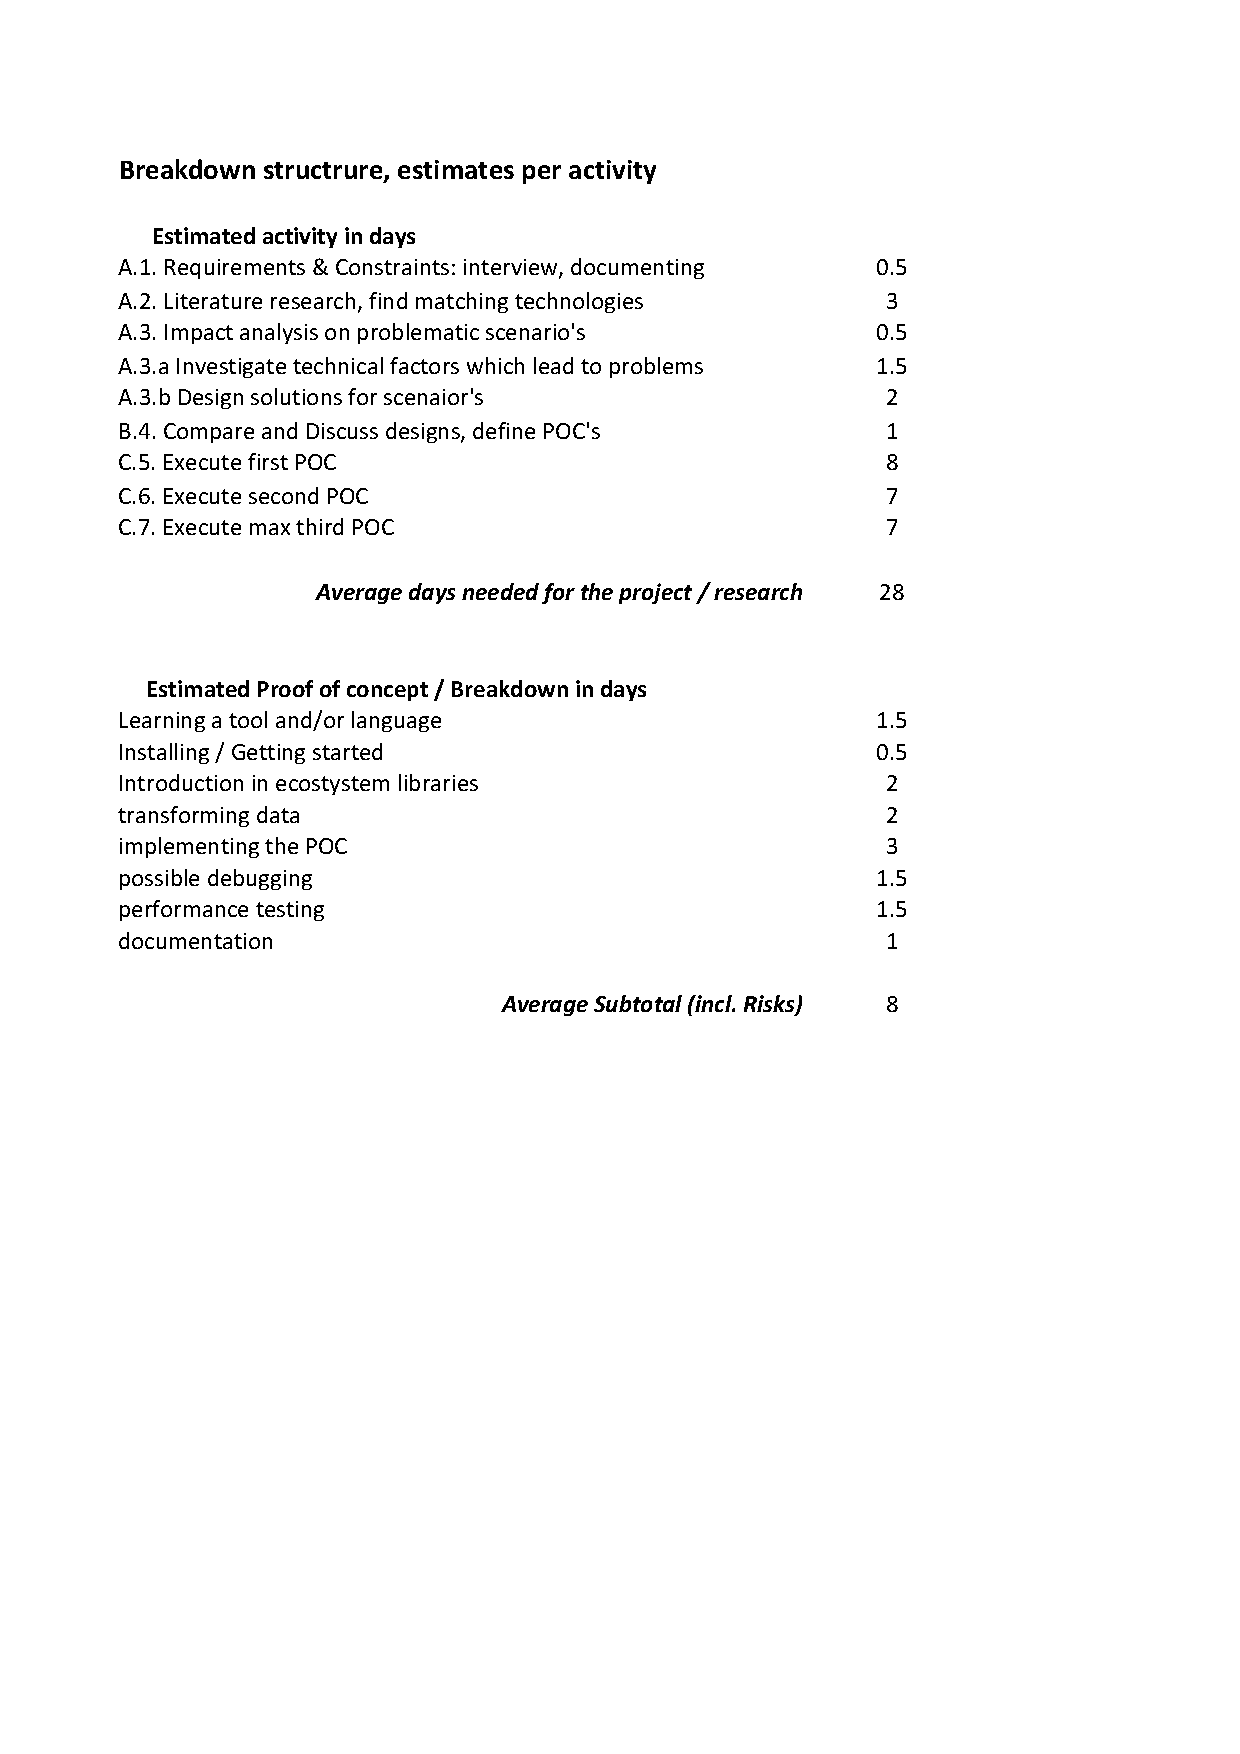
\includepdf[pages={1,2}]{appendix/planning-appendix-A.pdf}


\printbibliography

\end{document}